\section{Introducción}
\noindent Esta práctica consta de tres partes. En primer lugar, mediremos la diferencia de potencial que hay en una pila, seguidamente mediremos los potenciales de diferentes pares redox frente a un electrodo de referencia y, finalmente, realizaremos ensayos redox cualitativos.

\vspace{0.4cm}
\section{Inventario}
Para esta práctica hemos usado:

\begin{multicols}{2}
    \begin{itemize}
        \item Vasos de precipitados
        \item Papel de filtro
        \item Tijeras
        \item Espátulas metálicas
        \item Multímetro (y cables)
        \item Electrodos (grafito, oro y cinc)
        \item Electrodo de referencia (\ce{AgCl}/\ce{Ag})
        \item Polvo de cinc y cobre
        \item Lijas de grafito, cobre y cinc
        \item \ce{CuSO4} $1M$
        \item \ce{FeCl3} $0.1M$ y \ce{FeCl3} $0.1M$
        \item \ce{ZnSO4} $1M$
        \item \ce{I2} + \ce{KI} $1M$
        \item \ce{KI} $0.1M$
        \item \ce{KSCN}
        \item \ce{NH3} concentrado
    \end{itemize}
\end{multicols}

\begin{figure}[H]
    \centering
    \hspace*{-3cm}
        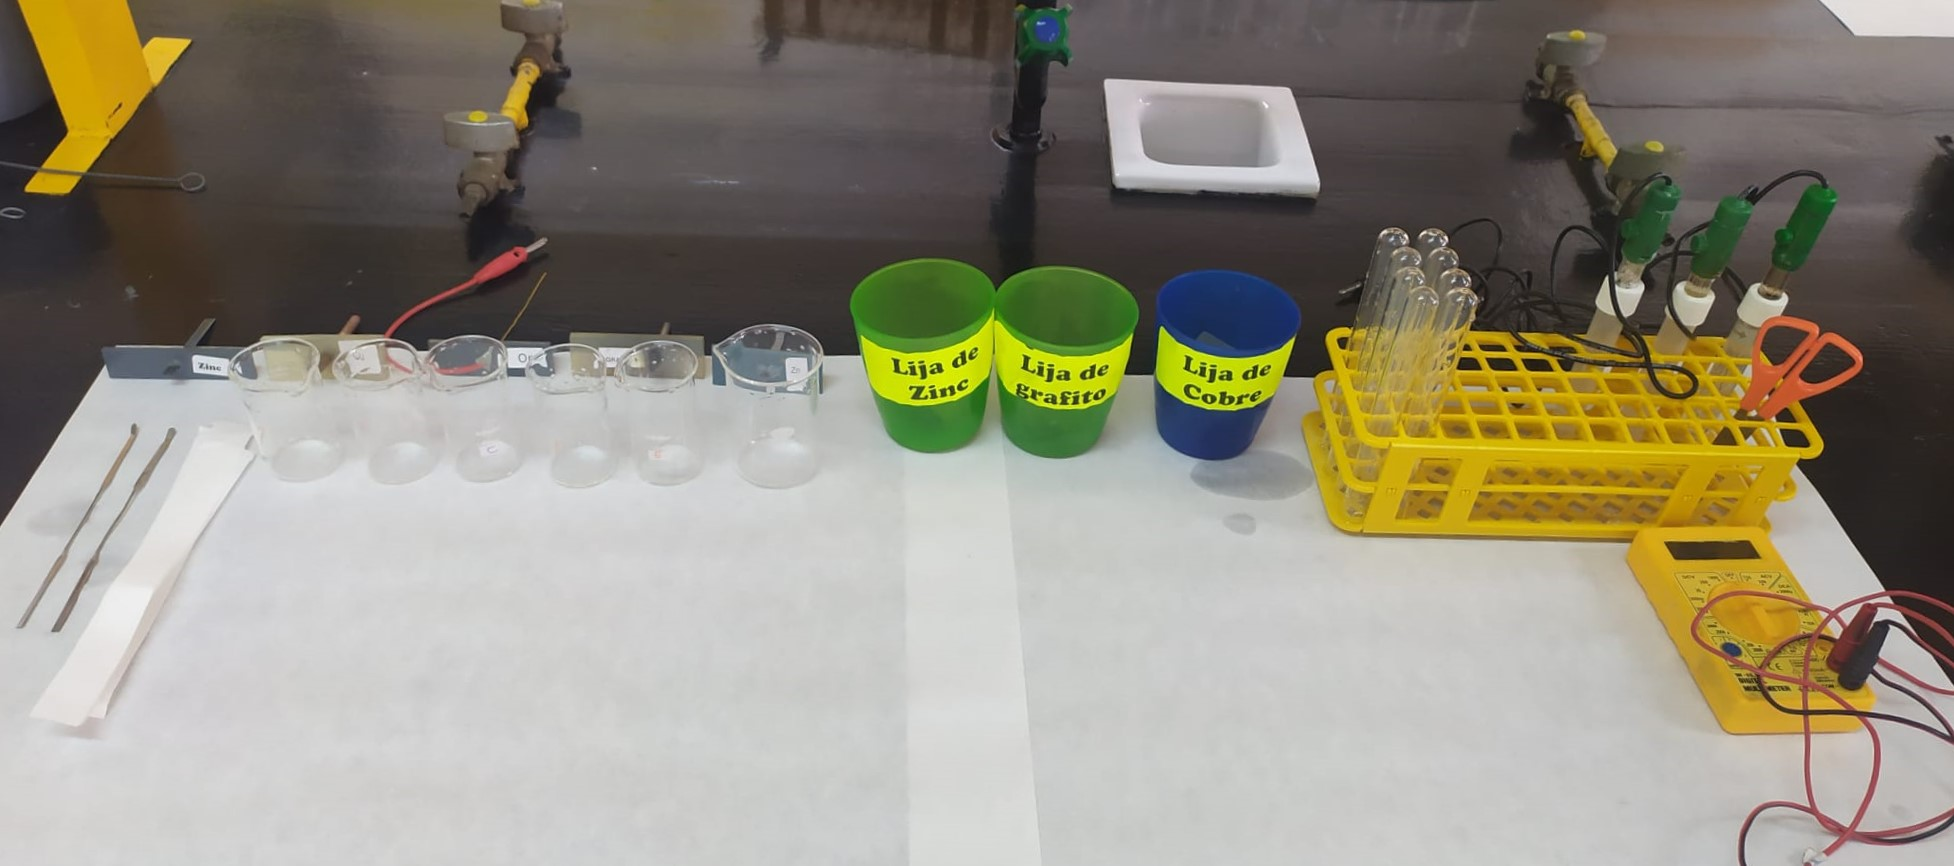
\includegraphics[scale = 0.2]{prac5/Material.jpeg}
        \includegraphics[scale = 0.087]{prac5/Líquidos_empleados.jpeg}
    \hspace*{-3cm}
    \caption{Material utilizado a lo largo de la práctica}
\end{figure}

\clearpage

\section{Procedimiento}
\subsection{Medición de la diferencia de potencial de una pila}
\noindent Colocaremos las 4 soluciones de 40 \si{ml} en vasos de precipitado distintos, marcándolas como A,B,C y D:
\begin{enumerate}[A -]
\item CuSO4 1M
\item Disolución clorhídrica 0,1 M en FeCl3 y FeCl2
\item ZnSO4 0,1 M
\item I2 + KI 0,1 M
\end{enumerate}

\noindent Ahora, vamos a crear diferentes pilas según los pares redox que conectemos y los electrodos que utilicemos:

\begin{enumerate}
\item A con electrodo de Cu y B con electrodo de grafito
\item A con electrodo de Cu y B con electrodo de Au
\item A con electrodo de Cu y C con electrodo de Zn
\item A con electrodo de Cu y D con electrodo de grafito
\item B con electrodo de grafito y C con electrodo de Zn
\item B con electrodo de Au y D con electrodo de grafito
\item C con electrodo de Zn y D con electrodo de grafito
\end{enumerate}

\noindent Anotamos los diferentes potenciales obtenidos para los pares de disoluciones A-D:

\begin{table}[H]
\centering
\begin{tabular}{ccc}
\rowcolor[HTML]{9698ED} 
\textbf{Pila} & \textbf{$\Delta V_{\text{teórico}}$ (\si{V})} & \multicolumn{1}{l}{\cellcolor[HTML]{9698ED}\textbf{$\Delta V_{\text{experimental}}$ (\si{V})}} \\
\rowcolor[HTML]{DAE8FC} 
\textbf{B - A (grafito)} & $0.43$ & $0.41$ \\
\textbf{B - A (oro)} & $0.43$ & $0.42$ \\
\rowcolor[HTML]{DAE8FC} 
\textbf{B - C} & $1.53$ & $1.41$ \\
\textbf{B - D} & $0.23$ & $0.18$ \\
\rowcolor[HTML]{DAE8FC} 
\textbf{A - C} & $1.10$ & $0.94$ \\
\textbf{A - D} & $0.20$ & $0.23$ \\
\rowcolor[HTML]{DAE8FC} 
\textbf{C - D} & $1.30$ & $1.25$
\end{tabular}
\label{potencial}
\end{table}
\noindent Destacar como el electrodo de oro posee una menor resistencia eléctrica y por ello se acerca más al valor teórico.
\clearpage

\subsection{Medida de los potenciales de diferentes pares frente a un electrodo de
referencia}
\noindent Para realizar estas medidas, cogeremos el vaso de precipitados restante e
introduciremos 40 mL de una disolución saturada de cloruro de potasio, en la que
sumergiremos el electrodo de referencia \ce{AgCl/Ag}, conectándolo al polo negativo
de nuestro multímetro.\\\\
A continuación, formaremos 4 pilas nuevas, formadas cada una por la nueva
disolución y realizando combinaciones con las disoluciones A-D, con el fin de
medir cada uno de los potenciales.

\begin{table}[H]
\centering
\begin{tabular}{cc}
\rowcolor[HTML]{9698ED} 
\textbf{Disolución} & \textbf{$\Delta V$} \\
\rowcolor[HTML]{DAE8FC} 
\textbf{A} & $0.08$ \\
\textbf{B} & $0.44$ \\
\rowcolor[HTML]{DAE8FC} 
\textbf{C} & $-0.9$ \\
\textbf{D} & $0.32$
\end{tabular}
\caption{Electrodo de referencia}
\label{referencia}
\end{table}

\subsection{Ensayos redox cualitativos}
\noindent Mediante el uso de tubos de ensayo y diferentes reactivos sólidos, llevamos a cabo estas reacciones, anotando los cambios observados.
\begin{enumerate}
\item 20 gotas de la disolución de FeCl3 0,1 M con 20 gotas de KI 0,1 M
\item 20 gotas de KI 0,1 M con 20 gotas de ZnSO4 0,1 M
\item Polvo de Zn con 20 gotas de la disolución de FeCl3 0,1 M. En este caso, ensayamos la presencia de iones Fe3+ con unas gotas de KSCN 0,1 M
\item 20 gotas de la disolución de FeCl3 con unas gotas de KSCN y polvo de Zn
\item Polvo de Zn con 20 gotas de la disolución de CuSO4. Ensayamos la presencia de iones Cu2+ con unas gotas de disolución concentrada de NH3.
\item 20 gotas de CuSO4 con 20 gotas de ZnSO4
\item Polvo de Zn con 20 gotas de una disolución de HCl 6M
\item Polvo de Cu con 30 gotas de una disolución de HCl 6M. Ensayamos la presencia de iones Cu2+ con unas gotas de disolución concentrada de NH3
\end{enumerate}


\clearpage
\section{Cuestiones}
\noindent\textcolor{BlueViolet}{\textbf{\textit{a) Exprese mediante ecuaciones los procesos redox que tienen lugar en cada una de las pilas formadas en el apartado 1. De acuerdo con los potenciales y polaridades observados, ordene los diferentes pares redox según su poder oxidante creciente.}}}\\
\begin{enumerate}
\item A con electrodo de Cu y B con electrodo de grafito \\
    Cátodo - $(\ce{2Fe^{3+} + 3e^- <=> 2Fe^{2+}})\cdot 2$ \\
    Ánodo  - $(\ce{Cu <=> Cu^{2+} + 2e^-})\cdot 3$ \\
    $\overline{\ce{4Fe^{3+} + 3Cu <=> 3Cu^{2+} + 4Fe^{2+}}}$
\item A con electrodo de Cu y C con electrodo de Zn \\
    Cátodo - $\ce{2Fe^{3+} + 2e^- <=> 2Fe^{2+}}$ \\
    Ánodo  - $\ce{Zn <=> Zn^{2+} + 2e^-}$ \\
    $\overline{\ce{2Fe^{3+} + Zn <=> Zn^{2+} + 2Fe^{2+}}}$
\item A con electrodo de Cu y D con electrodo de grafito \\
    Cátodo - $\ce{Cu^{2+} + 2e^- <=> Cu}$ \\
    Ánodo  - $\ce{2I^- <=> I2 + 2e^-}$ \\
    $\overline{\ce{Cu^{2+} + 2I^- <=> Cu + I2}}$
\item B con electrodo de grafito y C con electrodo de Zn \\
    Cátodo - $(\ce{Fe^{3+} + e^- <=> Fe^{2+}})\cdot 2$ \\
    Ánodo  - $\ce{Zn <=> Zn^{2+} + 2e^-}$ \\
    $\overline{\ce{2Fe^{3+} + Zn <=> 2Fe^{2+} + Zn^{2+}}}$
\item B con electrodo de Au y D con electrodo de grafito \\
    Cátodo - $(\ce{Fe^{3+} + e^- <=> Fe^{2+}})\cdot 2$ \\
    Ánodo  - $\ce{2I^- <=> I2 + 2e^-}$ \\
    $\overline{\ce{2Fe^{3+} + 2I^- <=> 2Fe^{2+} + I2}}$
\item C con electrodo de Zn y D con electrodo de grafito \\
    Cátodo - $\ce{I2 + 2e^- <=> 2I^-}$ \\
    Ánodo  - $\ce{Zn <=> Zn^{2+} + e^-}$ \\
    $\overline{\ce{I2 + Zn <=> 2I^- + Zn^{2+}}}$
\end{enumerate}
\clearpage

\noindent\textcolor{BlueViolet}{\textbf{\textit{b) Ordene los pares de mayor a menor potencial de acuerdo con las medidas del apartado 2. y compare el resultado con la ordenación establecida en el apartado 1. Compare los valores de potencial obtenidos en el apartado 2 con los esperados según los datos del Handbook.}}}\\\\
\noindent Siguiendo los datos acerca de los potenciales que hemos tomado en la tabla \ref{referencia}, podemos ordenar las pilas según el poder oxidante en sentido creciente:
\[\textbf{\boxed{\text{C <\ A <\ D <\ B}}}\]
Esta ordenación concuerda con la obtenida en la cuestión anterior, por lo que confirma la certeza de los datos obtenidos. Para asegurarnos más, comparamos con los datos existentes en el \textquote{\textit{CRC Handbook of Chemistry and Physics}}:
\begin{table}[H]
\centering
\begin{tabular}{ccc}
\rowcolor[HTML]{9698ED} 
\textbf{Reacción} & \textbf{$\Delta V_{\text{teórico}}$} & \cellcolor[HTML]{9698ED}\textbf{$\Delta V_{\text{experimental}}$} \\
\rowcolor[HTML]{DAE8FC} 
\textbf{A} & $-0.16$ & $+0.08$ \\
\rowcolor[HTML]{FFFFFF} 
\textbf{B} & $+0.77$ & $+0.44$ \\
\rowcolor[HTML]{DAE8FC} 
\textbf{C} & $-0.76$ & $-0.9$ \\
\textbf{D} & $+0.54$ & $+0.32$
\end{tabular}
\label{pot5}
\end{table}
\noindent\textcolor{BlueViolet}{\textbf{\textit{c) Discuta los resultados obtenidos en el apartado 3 en base a los valores de potencial obtenidos en los apartados anteriores. Escriba las ecuaciones correspondientes en los casos en los que hubo reacción.}}}

\begin{changemargin}{1.5cm}{0cm}
\noindent
\begin{enumerate}[\text{Reacción} 1 - ]
    \item El \ce{Fe^{3+}} se reduce y el \ce{I^-} se oxida. Se observa un color rojo en la reacción.\\
    \ce{2Fe^{3+} + 2I^- <=> 2Fe^{2+} + I2}
    \item El \ce{Zn^{2+}} se reduce y el \ce{I^-} se oxida. No es espontánea. \\
    \ce{Zn^{2+} + 2I^- <=> Zn + I2}
    \item Se observa color rojizo. Aparición de burbujas de gas.\\
    \ce{KSCN + FeCl3 + 5H2O -> [Fe(NCS)(H2O)5]^{2+} + 2Cl^- + KCl}
    \item El polvo de cinc precipita.
    \item No sucede nada, lo que implica una ausencia de iones \ce{Cu^{2+}}.
    \item No sucede nada.
    \item Se observa la aparición de burbujas de gas. Aumento de la temperatura.
    \item Se observa un coloro azul en la reacción al añadir \ce{NH3} \\
    \ce{Cu^{2+} + 4NH3 <=> Cu(NH3)4^{2+}}
\end{enumerate}
\end{changemargin}